% !TEX root = ../main.tex
% --+ 10.11 DIS +---------------------------------------------------------------
\begin{frame}{Deep Inelastic Scattering (DIS)}
    \label{10.11::dis}

    \begin{itemize}
        \item
            DIS refers to the scattering of an $e^-$ off a quark inside a nucleon.

        \item
            If we can detect the scattered $e^-$ and one of the scattered hadrons, we refer to the process as Semi Inclusive DIS (SIDIS).
    \end{itemize}

    \vspace{-12pt}
    \begin{columns}[onlytextwidth,T]

    \begin{column}{.49\linewidth}
        \begin{center}
            \begin{figure}[t]
                \centering{
                    \fbox{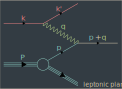
\includegraphics[width=\textwidth]{11dis_diagram.pdf}}
                }
            \end{figure}
        \end{center}
    \end{column}

    \begin{column}{.49\linewidth}
        \vspace{21pt}
        \small{\textit{
            \ef{Feynman diagram of DIS.}
            \begin{itemize}
                \vspace{6pt}
                \item
                    The nucleon and quark four-momenta are \eblue{$P$} and \eblue{$p$}, respectively.
                \vspace{6pt}
                \item
                    The initial and final four-momenta of the $e^-$ are \ered{$k$} and \ered{$k'$}.
                \vspace{6pt}
                \item
                    The momentum transferred to the hadron system is \egreen{$q = k - k'$}, from which we derive \egreen{$q^2 = -Q^2$}.
            \end{itemize}
        }}
    \end{column}

    \end{columns}
\end{frame}

% --+ 10.12 DIS +---------------------------------------------------------------
\begin{frame}{DIS: Kinematic Variables}
    \label{10.12::dis}

    \begin{itemize}
        \item
            Transferred momentum: \ef{$Q^2$} $= -(k - k')^2$ \ef{$\labeq 4E_bE'\sin^2(\theta_C/2)$}, where \ef{$E_b$} is the beam energy, and \ef{$E'$} and \ef{$\theta_C$} are the energy and angle of the scattered $e^-$.

        \item
            Virtual photon energy: \ef{$\nu \labeq E_b - E'$}.

        \item
            Hadron energy fraction: \ef{$z_h \labeq E_h/\nu$}, where \ef{$E_h$} is the hadron's energy.

        \item
            The hadron's transverse momentum \eorange{$p_T$} and the angle between the leptonic and hadronic planes \eorange{$\varphi_{PQ}$} can be understood in the figure.
    \end{itemize}

    \begin{center}
        \begin{figure}[t]
            \centering{
                \fbox{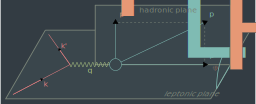
\includegraphics[width=0.8\textwidth]{12dis_planes.pdf}}
            }
        \end{figure}
    \end{center}
\end{frame}

% --+ 10.13 HADRONIZATION +-----------------------------------------------------
\begin{frame}{Hadronisation}
    \label{10.13::hadronisation}

    \vspace{12pt}

    \begin{itemize}
        \item
            \ef{Hadronisation} is the process in which quarks and gluons form hadrons.

        % \vspace{6pt}
        % \item
        %     The process is characterised by its \ef{Production Time} and \ef{Formation Time}.

        \vspace{12pt}
        \item
            The primary observable is the \ef{multiplicity of hadrons produced in nuclei of varying density}.
    \end{itemize}

    \vspace{-12pt}

    \begin{center}
        \begin{figure}[t]
            \centering{
                \fbox{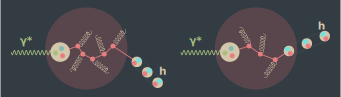
\includegraphics[width=\textwidth]{13hadronisation.pdf}}
            }
        \end{figure}
    \end{center}

    % NOTE. Maybe one of figures with tons of lines and hadrons going everywhere would be better here?
\end{frame}
